\documentclass[fleqn]{jbook}
\usepackage{physpub}

\begin{document}

\begin{question}{専攻 問題8}{}

\begin{subquestions}
\SubQuestion
Linus Paulingは2つのアミノ酸(H$_2$N-C$\alpha$R$_j$H-COOH,C$\alpha$は中心的位置にある炭素原子であり、$\alpha$-炭素と呼ばれ、R$_j$はアミノ酸によって異なる側鎖を表す)がペプチド結合(-CO-NH-)を通じて共有結合してできたジペプチドの立体的原子構造を解析した。その結果、CONHの4原子が一平面上にあるという興味ある意外な事実を掴んだ。彼はタンパク質分子の中でも、この4原子は常に同一平面上にあると考え、α-ヘリックスやβ-シートのモデルを提唱した。

\begin{subsubquestions}
\SubSubQuestion
どのような実験法を用いて、ジペプチドの立体的原子構造を明らかにしたかを3行以内で述べよ。(事実を知らない場合は、推察でよいが、推察の筋道を述べよ。)

\SubSubQuestion
Paulingは、CONHの4原子が一平面にあるという事柄を裏付ける別に事実にも気付いていた。それは何か。その事実と4原子が一平面上にあるという事柄の関係を述べよ。(事実を知らない場合は、推察でよいが、推察の筋道を述べよ。)
\end{subsubquestions}

\SubQuestion

α-ヘリックスの構造を考えよう。α-ヘリックスの中ではアミノ酸残基(-HN-C$\alpha$R$_j$H-CO-)がラセン対称性を持って規則的に並んでいる。各α-炭素を貫く右巻きのラセンのピッチは、0.54 nmであり、ラセン軸方向をz軸にとると、j番目のα-炭素のz座標は0.15 j (nm)である。この様な構造はz軸方向に並んだ周期cの一次元結晶と見なせる。

\begin{subsubquestions}
\SubSubQuestion
上記の数値を用いて、周期$c$(True pitchと呼ばれる)を求めよ。

\SubSubQuestion
α-ヘリックスの立体構造を安定化すると考えられる非共有結合について、考えられるだけの種類を挙げ、3行以内で述べよ。(事実を知らない場合は、推察でよいが、推察の筋道を述べよ。)
\end{subsubquestions}

\SubQuestion
α-ヘリックスからなるタンパク質のうち一群のファミリーがあり、それらのタンパク質ではヘプタッド・モチーフ(Heptad motif)がある。これは、アミノ酸配列が7個を周期的に繰り返し、......abcdefgabcdefgabcdefg....となっており、ここでaとdは疎水性アミノ酸である。

\begin{subsubquestions}
\SubSubQuestion
このモチーフをもつα-ヘリックスのなかでの疎水性アミノ酸残基の三次元的配置を図示し、その特徴を述べよ。

\SubSubQuestion
このモチーフをもつα-ヘリックスが二分子あると、水溶液中では互いに結合して、特徴ある四次構造を形成する。その特徴を述べよ。(事実を知らない場合は、推察でよいが、推察の筋道を述べよ。)
\end{subsubquestions}

\end{subquestions}
\end{question}
\begin{answer}{専攻 問題8}{}
\begin{subanswers}
\SubAnswer

 \begin{subsubanswers} 
  \SubSubAnswer
    ジペプチドの結晶に単一波長のX線を当て、散乱される様子を写真で調べ、
   電子密度図を得、それから原子の立体的位置を決める。
%
   \SubSubAnswer   
        ペプチドは右図のような共鳴構造をとる。 C-Nが二重結合性をもつた
       めに、この結合を軸として回転することができず、CONHの4原子が一平
       面内にある。
     \bigskip
   
   \begin{center}
   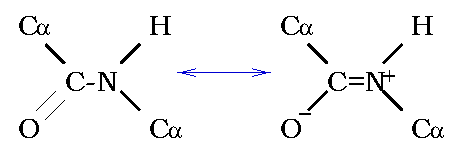
\includegraphics[clip,height=20mm,width=75mm]{1997phy8-1.eps}
   \end{center}
   \end{subsubanswers}

%
\SubAnswer

  \begin{subsubanswers}
    \SubSubAnswer
\[
c=\frac{0.54[{\Unit{nm}}]}{0.15[{\Unit{nm}}]}=3.6
\]

    \SubSubAnswer

     n番目のアミノ酸のカルボニル酸素原子とn+3番目のアミノ酸残基の水素
原子とで水素結合することで構造を安定化する。同じ電荷を持つ残基が少なけ
れば(互いに異なる電荷をもつ残基が並べば)相互に反発しないので安定であ
る。
    \end{subsubanswers}
%
\SubAnswer
\parbox[t]{130mm}{
  \begin{subsubanswers}
    \SubSubAnswer
   疎水的アミノ酸残基が同じ側に並ぶのが特徴である。 
    \SubSubAnswer
(i)で示した螺旋状の疎水性アミノ酸が2分子間で近接し、各々がねじれて巻き付く
ことでコイルドコイルを形成し安定化する。
  \end{subsubanswers}}\parbox[t]{30mm}{
\begin{center}
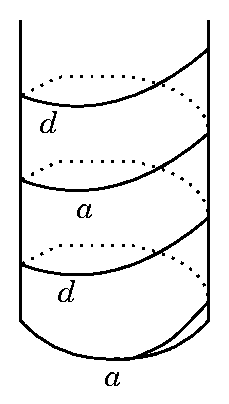
\includegraphics[clip,height=40mm,width=20mm]{1997phy8-2.eps}
\end{center}
}
%
\end{subanswers}
\end{answer}

\end{document}
